\documentclass[11pt]{article}
\usepackage[a4paper,margin=2.6cm]{geometry}
\usepackage[T1]{fontenc}
\usepackage[utf8]{inputenc}
\usepackage{lmodern}
\usepackage{amsmath,amssymb,amsthm}
\usepackage{microtype}
\usepackage{tikz}
\usetikzlibrary{arrows.meta,calc,positioning}
\usepackage[hidelinks]{hyperref}
\usepackage{enumitem}
\setlist{itemsep=2pt,topsep=4pt}

\newtheorem*{result}{Result}
\newcommand{\R}{\mathbb{R}}
\newcommand{\iv}[1]{[#1]}

\title{\vspace{-1.2cm}The maximum size of an almost-equidistant set\\ in $\R^4$ is twelve\\[4pt]
\large A computer-assisted resolution of a conjecture of\\ Balko, P\'or, Scheucher, Swanepoel and Valtr}
\author{}
\date{August 5, 2026}

\begin{document}
\maketitle
\vspace{-1.4cm}

\section*{Background}

A finite set of points in $\R^d$ is \emph{almost equidistant} if among any
three of its points, some two are at unit distance. Let $f(d)$ denote the
largest size of an almost-equidistant set in $\R^d$. Classically $f(2)=7$
(the Moser spindle, uniqueness due to Talata), and
\[
  f(3)=10,
\]
proved by \textbf{Bernadett Gy\"orey} in her 2004 master's thesis
\cite{Gyorey} (supervised by Istv\'an Talata), together with the uniqueness of
the extremal ten-point configuration --- two unit tetrahedra with two reflected
vertices, one copy rotated about the axis through the reflected points. This
result is Theorem~2 of the paper of Balko, P\'or, Scheucher, Swanepoel and
Valtr \cite{BPSSV}, who reproved it with computer assistance, established
\[
  12 \le f(4) \le 13,
\]
and conjectured (their Conjecture~1) that $f(4)=12$. The lower bound comes from
the $(2d{+}4)$-point generalization of the ten-point configuration; the upper
bound from their enumeration of candidate graphs. The gap has remained open.

\begin{result}
$f(4) = 12$. Conjecture~1 of \cite{BPSSV} holds
(computer-assisted proof; see the caveats below).
\end{result}

\section*{Reduction}

Following \cite{BPSSV}, the unit-distance graph of a hypothetical
thirteen-point almost-equidistant set in $\R^4$ must be an \emph{abstract
almost-equidistant graph}: a graph on 13 vertices with no independent set of
size~3, no $K_6$, and no $K_{1,3,3}$. There are exactly \textbf{59} such
graphs. We re-enumerated them independently; our counts agree with Table~3 of
\cite{BPSSV} at every order ($7$, $14$, $37$, $97$, $316$, $934$, $2362$,
$2814$, $944$, $\mathbf{59}$, $4$, $1$, $1$, $0$ for $n=4,\dots,17$). Thus
$f(4)=13$ if and only if one of these 59 graphs admits a \emph{realization}: an
assignment of \emph{13 distinct} points of $\R^4$ placing every edge at
distance exactly~$1$ (non-edges are unconstrained). We certified that
\textbf{none of the 59 graphs admits such a realization}. Appendix~A details
the enumeration, Appendix~B the certified decision procedure, and Appendix~C
the search orchestration.

\section*{Method (overview)}

For each graph, a branch-and-prune search over \emph{rigorous interval
arithmetic} (outward-rounded IEEE double precision) explores all possible
placements up to congruence:

\begin{itemize}
\item a seed clique ($K_5$ or $K_4$, a unit simplex, rigid up to congruence)
      is placed with exact interval enclosures;
\item a vertex with $\ge 4$ placed neighbours lies on the intersection of four
      unit spheres --- at most two points, giving a binary branch tree, with
      enclosures contracted by the Krawczyk operator and surplus neighbours
      acting as certified pruning constraints;
\item a vertex with exactly $3$ placed neighbours lies on a circle,
      parametrized exactly and subdivided adaptively; near-tangent
      configurations are resolved by a one-dimensional subdivision along the
      root segment.
\end{itemize}

A branch is discarded only when an interval certifiably excludes a required
value, so eliminating \emph{all} branches proves non-realizability.

A key subtlety --- echoing \S3.5 (``multiple points'') of \cite{Gyorey} --- is
that these graphs \emph{do} admit degenerate realizations in which some
non-adjacent vertices coincide; such configurations have fewer than 13 distinct
points and are irrelevant, but they satisfy every edge constraint and would
survive naive pruning. Two certified rules (Appendix~B.6) discard branches on
which coincidence is \emph{forced}.

\emph{Validation.} The engine kills the ten-vertex graph proved non-realizable
in Lemma~12 of \cite{BPSSV}, and does \emph{not} kill the realizable
cross-polytope graph $K_{2,2,2,2}$ --- for which it isolates exactly the two
mirror-image unit cross-polytopes. During development the engine was
maintained in two independent implementations (a Python reference and a C
production version, roughly $1000\times$ faster), which produced identical
search trees node-for-node on matched instances; the reproduction package
ships the C implementation. The C engine's determinism was additionally
verified \emph{across platforms}: on a matched battery of instances ---
including full searches of both control graphs --- Apple clang/libm on ARM64
(M2 Pro, macOS 14.5), MSVC/UCRT on x86-64, and LLVM clang/UCRT on x86-64
(Ryzen 9950X3D, Windows 11) produce bit-identical search trees, node and
unresolved-cell counts agreeing exactly both on zero-circle instances
(exercising only correctly rounded basic operations) and on circle-bearing
instances (additionally exercising the padded library $\cos/\sin$
enclosures). During development a genuine bug in the circle
parametrization (a Gram--Schmidt error) was caught by manual inspection of a
single cell; a runtime canary --- aborting the computation if a parametrized
circle point ever violates its own defining constraint --- was added in
response, and every result predating the fix was discarded and recomputed.

\emph{Execution.} Fifty-six of the 59 graphs die quickly (milliseconds to
minutes). The three hardest --- including the unique graph requiring a
two-parameter search --- were finished by partitioning the circle parameter
into certified slices computed in parallel on 12 CPU cores; one graph exhibited
a degenerate tangency channel specific to the chosen elimination order and was
instead certified in full by an alternate order, for which all 24 slices
covering the whole circle die. In total: \textbf{zero surviving branches
anywhere}. Independent numerical optimization (Levenberg--Marquardt, 200
restarts per graph) corroborates the verdict: no graph comes close to
realizability (best residual $0.078$, versus $10^{-31}$ for a realizable
control).

\section*{Caveats and reproducibility}

The proof is computer-assisted. It assumes IEEE-754 correctly-rounded floating
point arithmetic and standard-library $\cos/\sin$ accurate to within 8 units in
the last place (padded accordingly), and the correctness of the verification
engine described in Appendix~B. A self-contained reproduction package (all
source code, the enumerated graphs, and a one-command driver) accompanies this
note, so that the computation can be replicated or re-implemented independently
--- which we would warmly encourage before the result is treated as
established.

With $f(2)=7$, $f(3)=10$ \cite{Gyorey}, and now $f(4)=12$, the first four
values of $f$ are settled.

\begin{thebibliography}{9}\small
\bibitem{Gyorey} B.~Gy\"orey,
\emph{Diszkr\'et metrikus terek be\'agyaz\'asai}, Master's thesis,
E\"otv\"os Lor\'and University, Budapest, 2004.

\bibitem{BPSSV} M.~Balko, A.~P\'or, M.~Scheucher, K.~Swanepoel, P.~Valtr,
\emph{Almost-equidistant sets}, Graphs and Combinatorics \textbf{36} (2020),
729--754. arXiv:1706.06375.

\bibitem{KMS} A.~Kupavskii, N.~Mustafa, K.~Swanepoel,
\emph{Bounding the size of an almost-equidistant set in Euclidean space},
Combinatorics, Probability and Computing \textbf{28} (2019), 280--286.
\end{thebibliography}

\appendix

\section{Enumeration of the candidate graphs}
\label{app:enum}

\emph{(Implemented in \texttt{enumerate\_aeq.py}.)}
A graph $G$ is an abstract almost-equidistant graph in $\R^4$ if
(i)~$\alpha(G)\le 2$, i.e.\ the complement is triangle-free (this is the
almost-equidistance condition itself); (ii)~$G$ contains no $K_6$ (at most
$d{+}1=5$ points of $\R^4$ are pairwise at unit distance); and (iii)~$G$
contains no complete tripartite $K_{1,3,3}$ (Lemma~11 of \cite{BPSSV}).

\textbf{Generation.} Graphs are grown one vertex at a time from a single
vertex. When a graph on $n$ vertices is extended by a new vertex $v$, we may
assume $v$ has minimum degree in the extended graph: all three defining
properties are inherited by induced subgraphs, so every $(n{+}1)$-vertex
witness arises from deleting a minimum-degree vertex. Moreover
$\deg(v)\ge n-5$, because the non-neighbourhood of any vertex must induce a
clique (two non-adjacent non-neighbours would form an independent triple with
$v$), and cliques have size $\le 5$ by (ii). For each admissible neighbourhood
the three conditions are checked \emph{incrementally}, i.e.\ only for
configurations involving $v$: the non-neighbours of $v$ must be pairwise
adjacent; no $5$-clique of the parent may lie inside $N(v)$ (else a $K_6$);
and a $K_{1,3,3}$ through $v$ is detected by testing, for $v$ as the singleton
and for $v$ inside a triple, whether some triple $X\subseteq N(a)$ has at
least three common neighbours inside $N(a)\setminus X$ (a bitmask
intersection-popcount test).

\textbf{Isomorphism rejection.} Candidates are bucketed by the invariant
$\{(\deg u,\ \#\text{triangles at } u,\ \text{sorted neighbour degrees})\}_u$
and compared within buckets by a backtracking isomorphism search with degree
pruning.

\textbf{Verification.} Every generated graph is re-checked by independent,
non-incremental tests of (i)--(iii). The resulting counts match \cite{BPSSV}
Table~3 for every $n$ (the sequence quoted in the main text; in particular
there are $59$ graphs for $n=13$ and none for $n\ge 17$), and the counts of
\emph{minimal} graphs (those in which deleting any edge creates an independent
triple; an edge $uv$ is deletable iff $N(u)\cup N(v)\cup\{u,v\}$ is not the
whole vertex set) match their Table~2, e.g.\ $12$ minimal graphs on $13$
vertices. Although killing the $12$ minimal graphs would suffice (every
realization of an abstract graph restricts to one of a spanning minimal
subgraph), we certified all $59$.

\section{The certified decision procedure}
\label{app:engine}

\emph{(Implemented in \texttt{ckernel.c}, compiled and driven by
\texttt{cdriver.py}; the exact seed enclosures of \S B.2 are constructed in
\texttt{ival.py}.)}

\subsection{Interval arithmetic}
All geometry is computed in interval arithmetic over IEEE doubles with
\emph{outward rounding}: after each basic operation ($+,-,\times,/$,
$\sqrt{\ }$, which IEEE-754 rounds correctly), the bounds are widened by one
ulp via \texttt{nextafter}. Library $\cos/\sin$ are additionally padded by $8$
ulp and interval extrema at multiples of $\pi$ are handled explicitly. The
invariant throughout: \emph{every quantity's interval contains the exact real
value for every real configuration represented by the current branch}. A
constraint is violated --- and the branch discarded --- only when its interval
excludes the required value entirely.

\subsection{Normalization and seeds}
Every realization can be moved by an isometry so that a chosen clique
($K_5$ if present, else $K_4$; both exist in all $59$ graphs) occupies the
canonical unit simplex
\[
u_0=0,\quad u_1=e_1,\quad u_2=\bigl(\tfrac12,\tfrac{\sqrt3}{2},0,0\bigr),\quad
u_3=\bigl(\tfrac12,\tfrac{\sqrt3}{6},\tfrac{\sqrt6}{3},0\bigr),\quad
u_4=\bigl(\tfrac12,\tfrac{\sqrt3}{6},\tfrac{\sqrt6}{12},\tfrac{\sqrt{10}}{4}\bigr),
\]
placed as exact interval enclosures. (For a $K_4$ seed both mirror images are
explored by the branching itself.)

\subsection{Sphere placements}
If $v$ has placed neighbours $p_0,\dots,p_{k-1}$ with $k\ge4$, subtracting the
sphere equations pairwise yields the linear system
$2(p_i-p_0)\cdot x=\lVert p_i\rVert^2-\lVert p_0\rVert^2$ ($i=1,2,3$), solved
by interval Gauss--Jordan elimination with mignitude pivoting; the solution set
is a line $x=x_p+t\,n$, and substituting into $\lVert x-p_0\rVert^2=1$ gives a
quadratic $at^2+bt+c=0$. If its discriminant interval is negative the branch
dies; if it straddles zero the two roots are returned as one merged enclosure
(see B.5); otherwise two root enclosures give a binary branch. Each candidate
is contracted by the \emph{Krawczyk operator}
\[
K(X)=m-Y F(m)+\bigl(I-Y\,J(X)\bigr)(X-m),
\]
where $m$ is the midpoint box, $F$ the four sphere residuals, $J$ their
interval Jacobian, and $Y$ a floating-point approximate inverse of the midpoint
Jacobian (the best-conditioned $4$-subset of neighbours is chosen by maximal
$|\det|$). $K(X)\cap X=\emptyset$ certifiably kills the branch; otherwise the
intersection is a valid, usually much tighter, enclosure. All remaining placed
neighbours act as extra certified constraints. After each placement inside a
circle cell, a Gauss--Seidel sweep re-contracts the neighbourhood
(constraints propagate backwards as well as forwards).

\subsection{Circle placements}
If $v$ has exactly three placed neighbours $p_0,p_1,p_2$, the solution set of
the three unit-sphere equations is a circle: its centre $c$ (the circumcentre
of $p_0,p_1,p_2$ in their affine plane) solves a $2\times2$ interval system,
its radius is $r=\sqrt{1-R^2}$ with $R=\lVert c-p_0\rVert$ (negative
$1-R^2$ kills the branch), and an orthonormal basis $u,w$ of the orthogonal
complement of the plane is obtained by interval Gram--Schmidt. Then
$x(\theta)=c+r(\cos\theta\,u+\sin\theta\,w)$, $\theta\in[0,2\pi)$, and
enclosures of $\cos,\sin$ over a $\theta$-cell give an enclosure of all circle
points of that cell. Cells are bisected adaptively: a cell whose subtree is not
entirely killed is split until a width floor is reached (surviving cells are
reported, never dropped). A runtime canary aborts the whole computation if a
circle point ever fails its own defining constraints --- a guard against
implementation error, not a mathematical step.

\subsection{Near-tangent placements}
When the quadratic's discriminant straddles zero (two roots merging), the root
enclosure degenerates to a segment $x_p+t\,n$, $t\in\iv{t}$. Inside
sufficiently refined circle cells this segment is subdivided in $t$ like a
one-dimensional cell stage, which separates the near-coincident and
mirror-image solution regimes that a single fat box cannot distinguish.

\subsection{Distinctness: discarding forced coincidences}
\label{app:coinc}
The candidate graphs admit \emph{degenerate} edge-exact configurations with
coincident non-adjacent vertices (fewer than 13 distinct points). Two rules
discard branches that cannot contain an \emph{injective} realization; both
only ever discard, never affect kill soundness.

\emph{Rule 1 (root separation).} Let $u\not\sim v$ with overlapping boxes, and
let $Q$ be four placed common neighbours. In any true solution both $x_u$ and
$x_v$ solve the $Q$-sphere system, which has at most two solutions --- the two
roots above. If the two root enclosures are disjoint and the boxes of $x_u$
and $x_v$ meet the \emph{same single} root enclosure, then $x_u=x_v$ in every
true solution of the branch, which therefore contains no 13-distinct-point
realization. (If either box meets neither root, the branch is empty outright.)

\emph{Rule 2 (bisector hyperplane).} If $x_u\ne x_v$ and $w$ is a common
neighbour, then $\lVert x_w-x_u\rVert=\lVert x_w-x_v\rVert=1$ places $x_w$ on
the perpendicular bisector hyperplane of $x_u x_v$. Hence if five placed
common neighbours have certifiably nonzero affine volume (an interval
$4\times4$ determinant), no hyperplane contains them all and $x_u=x_v$ is
forced.

Both rules are applied at placement time and again as a filter at complete
leaves. Together with the branch elimination they yield: \emph{if every branch
of the search dies or is discarded, the graph admits no realization with 13
distinct points.} A cell that can neither be killed nor discarded at the width
floor is reported as a survivor; the final computation has none.

\section{Search orchestration: slicing and decompositions}
\label{app:orch}

\emph{(Implemented in \texttt{reproduce.py}; C driver \texttt{cdriver.py}.)}

\subsection{Elimination orders}
An \emph{elimination order} fixes the seed clique and the sequence of vertex
placements; each next vertex has $\ge4$ (sphere step) or exactly $3$ (circle
step) already-placed neighbours. Orders are generated greedily,
\emph{circle-late}: the placed set is closed under sphere steps before a
circle vertex is chosen (several tie-breaking heuristics give a small pool of
distinct decompositions per graph). The order affects only the shape and cost
of the search tree, never the soundness of a verdict; hence \emph{any} single
order whose search is fully killed certifies the graph.

\subsection{Slicing the circle parameter}
The engine accepts a restriction of the \emph{first} circle stage to a
subinterval $[a,b]\subseteq[0,2\pi]$. If a family of closed slices covers
$[0,2\pi]$ and each sliced search is fully killed, the graph is certified:
every hypothetical realization has some $\theta\in[0,2\pi]$ and falls in some
slice. Slices are independent, so they parallelize perfectly across cores.

\subsection{Recursive refinement}
Each slice is run with a node budget. A slice that exceeds its budget (or
reports survivors) is split into $8$ subslices and retried. Empirically this
is the dominant accelerator: with finer initial slices the engine's very first
cells are already narrow enough for immediate certified kills, avoiding the
repeated re-exploration that adaptive splitting of coarse cells entails ---
pieces that ran for hours at coarse slicing die in milliseconds two refinement
levels down. Fifty-six graphs need no slicing at all; two need one or two
levels; the graph with two circle stages (a two-parameter search) needed three
levels on part of its range. The driver therefore starts two-parameter
searches directly at fine initial slicing.

\subsection{Alternate decompositions}
One graph exhibits, under its default decomposition, an
\emph{identically-degenerate tangency channel}: along a narrow $\theta$-arc
the discriminant of the relevant sphere systems vanishes identically, two
vertex pairs coincide exactly (a degenerate configuration family), and the
coincidence rules of \S B.6 are structurally inconclusive there (merged roots;
vanishing affine volumes). Rather than analyse the channel, the driver races
all candidate decompositions concurrently: a different elimination order
re-parametrizes the geometry, the degenerate family no longer sits at a
tangency of the new parametrization, and the standard machinery certifies all
$24$ slices of the full circle directly. The final certificate for that graph
rests entirely on the alternate decomposition and is self-contained.

\subsection{Reproduction}
The package provides: \texttt{enumerate\_aeq.py} (Appendix~A; also verifies
all published counts), \texttt{ckernel.c} (the certified engine, Appendix~B)
with \texttt{cdriver.py}/\texttt{ival.py} (compilation, seed enclosures,
elimination orders), the graph list \texttt{aeq\_d4\_n13.json}, and
\texttt{reproduce.py}, which runs the two validation controls (Lemma-12 graph
killed; cross-polytope graph preserved) and then certifies all $59$ graphs by
the strategy above. The kernel compiles automatically (any C compiler on
POSIX; MSVC, clang or gcc on Windows); there are no further dependencies
beyond Python~$\ge$~3.9. A full run takes on the order of ten minutes on a
modern 16-core machine (the original campaign, which predated the driver's
fine-slicing default and concurrent-race cancellation, took on the order of
half a day for the hardest graphs on 12 cores); the computation is
deterministic, and was observed to reproduce bit-identical search trees
across the three compiler/libm/ISA stacks tested.

\section{The rotating-simplex construction: why thirteen fails and why
twelve is not unique}
\label{app:rotation}

The main result is a cardinality statement, not a congruence classification
of extremal sets.  This appendix records two geometric facts.  A tempting
$5+3+5$ modification already fails because its three middle points violate
almost equidistance.  By contrast, the valid $5+2+5$ construction has a
continuous twist parameter and is not unique up to congruence.

\subsection{Facet reflections of a unit \texorpdfstring{$4$}{4}-simplex}

Let $S=\{q_0,\dots,q_4\}$ be a regular unit $4$-simplex, translated so that
its centroid is the origin.  Its Gram matrix is
\[
 \langle q_i,q_i\rangle=\frac25,
 \qquad
 \langle q_i,q_j\rangle=-\frac1{10}\quad(i\ne j).
\]
The centroid of the facet opposite $q_i$ is $-q_i/4$.  Reflecting $q_i$
through the affine hyperplane of that facet therefore gives the other apex
\[
 r_i=2\left(-\frac{q_i}{4}\right)-q_i=-\frac32q_i.
\]
Consequently,
\begin{equation}
 \lVert r_i-q_j\rVert=1\quad(j\ne i),
 \qquad
 \lVert r_i-r_j\rVert=\frac32\quad(i\ne j).
 \label{eq:reflected-apex-distances}
\end{equation}
The first identity is what makes reflected apices useful.  The second is the
obstruction below.

\subsection{The tempting \texorpdfstring{$5+3+5$}{5+3+5} set}

One might try to use the five vertices of $S$, three reflected apices
$r_0,r_1,r_2$, and a rotated copy $\rho(S)$, for a total of thirteen points.
Let
\[
 A=\operatorname{aff}\{r_0,r_1,r_2\}.
\]
This is a plane in $\mathbb R^4$, so its orthogonal complement is
two-dimensional and an ordinary rotation about $A$ is well defined.  In fact,
the rotation required by the proposal really does exist.  Each of
$q_0,q_1,q_2$ has squared distance $5/12$ from $A$.  A rotation through an
angle $\theta$ moves all three of them by one exactly when
\[
 2\left(\frac5{12}\right)(1-\cos\theta)=1,
 \qquad\text{that is,}\qquad
 \cos\theta=-\frac15.
\]
Thus the failure is not an inability to choose a rotation.

It is instead immediate from \eqref{eq:reflected-apex-distances}: the three
points $r_0,r_1,r_2$ form an equilateral triangle of side $3/2$.  The triple
\[
 \{r_0,r_1,r_2\}
\]
contains no pair at unit distance, so the full thirteen-point set is not
almost equidistant.  Since the rotation fixes $A$ pointwise, it fixes all
three offending points and cannot repair this triple.  Figure~\ref{fig:five-three-five}
shows the obstruction schematically, and Figure~\ref{fig:three-apex-rotation}
shows that the proposed rotation itself is geometrically available.

\begin{figure}[htbp]
\centering
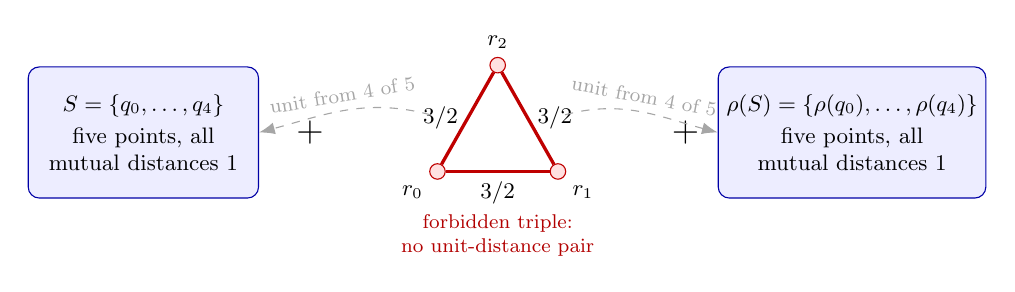
\begin{tikzpicture}[scale=0.9,transform shape,
  font=\small,
  simplex/.style={draw=blue!65!black,fill=blue!7,rounded corners=4pt,
                  minimum width=3.25cm,minimum height=1.85cm,align=center},
  rpoint/.style={circle,draw=red!75!black,fill=red!12,inner sep=2.2pt},
  badedge/.style={draw=red!75!black,very thick},
  note/.style={align=center,font=\footnotesize}
]
  \node[simplex] (S) at (-5,0)
    {$S=\{q_0,\ldots,q_4\}$\\[2pt]five points, all\\mutual distances $1$};
  \node at (-2.65,0) {\Large$+$};

  \coordinate (Rcentre) at (0,0);
  \node[rpoint,label=below left:$r_0$] (r0) at (-0.85,-0.55) {};
  \node[rpoint,label=below right:$r_1$] (r1) at (0.85,-0.55) {};
  \node[rpoint,label=above:$r_2$] (r2) at (0,0.95) {};
  \draw[badedge] (r0)--node[below] {$3/2$}(r1);
  \draw[badedge] (r1)--node[right] {$3/2$}(r2);
  \draw[badedge] (r2)--node[left] {$3/2$}(r0);
  \node[note,text=red!70!black] at (0,-1.45)
    {forbidden triple:\\no unit-distance pair};

  \node at (2.65,0) {\Large$+$};
  \node[simplex] (T) at (5,0)
    {$\rho(S)=\{\rho(q_0),\ldots,\rho(q_4)\}$\\[2pt]five points, all\\mutual distances $1$};

  \draw[-{Latex[length=2mm]},gray!70,dashed]
    ($(Rcentre)+(-0.95,0.25)$) to[out=165,in=15]
    node[above,sloped,note] {unit from $4$ of $5$} (S.east);
  \draw[-{Latex[length=2mm]},gray!70,dashed]
    ($(Rcentre)+(0.95,0.25)$) to[out=15,in=165]
    node[above,sloped,note] {unit from $4$ of $5$} (T.west);
\end{tikzpicture}
\caption{The attempted $5+3+5$ set, schematically.  The two blue boxes are
unit simplices.  Each reflected apex has the needed unit links to both
copies, but the three red points are mutually at distance $3/2$ and hence
form a forbidden triple.}
\label{fig:five-three-five}
\end{figure}

\begin{figure}[htbp]
\centering
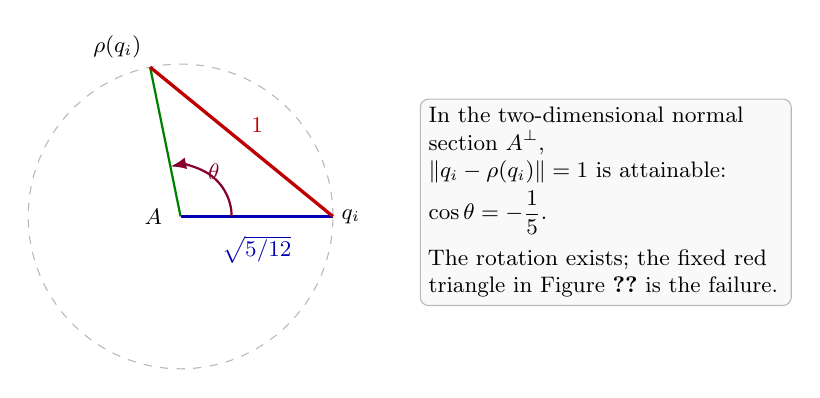
\begin{tikzpicture}[scale=0.9,transform shape,font=\small]
  \coordinate (O) at (0,0);
  \coordinate (Q) at (2.15,0);
  \coordinate (QP) at ({2.15*cos(101.537)}, {2.15*sin(101.537)});
  \draw[gray!55,dashed] (O) circle (2.15);
  \draw[blue!70!black,thick] (O)--node[below=4pt] {$\sqrt{5/12}$}(Q);
  \draw[green!50!black,thick] (O)--(QP);
  \draw[red!75!black,very thick] (Q)--node[above right] {$1$}(QP);
  \draw[-{Latex[length=2mm]},purple!70!black,thick]
    (0.72,0) arc[start angle=0,end angle=101.537,radius=0.72];
  \node[purple!70!black] at (0.47,0.63) {$\theta$};
  \node[left=4pt] at (O) {$A$};
  \node[right] at (Q) {$q_i$};
  \node[above left] at (QP) {$\rho(q_i)$};
  \node[draw=gray!55,fill=gray!5,rounded corners=3pt,align=left,
        text width=5.0cm] at (6.0,0.2)
    {In the two-dimensional normal section $A^\perp$,\\
     $\lVert q_i-\rho(q_i)\rVert=1$ is attainable:\\[2pt]
     $\displaystyle \cos\theta=-\frac15.$\\[5pt]
     The rotation exists; the fixed red triangle in
     Figure~\ref{fig:five-three-five} is the failure.};
\end{tikzpicture}
\caption{Normal cross-section of rotation about
$A=\operatorname{aff}\{r_0,r_1,r_2\}$.  The three exceptional vertices have
the same radius $\sqrt{5/12}$, so the displayed unit chords are attainable.}
\label{fig:three-apex-rotation}
\end{figure}

\subsection{The valid twelve-point set and its twist freedom}

The standard construction keeps only two reflected apices.  Choose
$r_0,r_1$, and an isometry $\rho$ fixing both of them and satisfying
\[
 \lVert q_0-\rho(q_0)\rVert
 =\lVert q_1-\rho(q_1)\rVert=1.
\]
Then
\[
 P=S\cup\rho(S)\cup\{r_0,r_1\}
\]
has $5+5+2=12$ distinct points and is almost equidistant.  Indeed, each
simplex copy is a unit clique.  Moreover, $r_k$ is at unit distance from
every point of either copy except $q_k$ and $\rho(q_k)$.  The only triple not
settled immediately by those unit edges would contain
$r_k,q_k,\rho(q_k)$, and its last two points are unit by the displayed
condition.  With only two reflected apices there is no three-point middle
set that could repeat the preceding obstruction.

There is, however, no uniqueness in dimension four.  To see the freedom
directly, translate the midpoint of $r_0r_1$ to the origin and put
\[
 c=\frac{q_0+q_1}{2},
 \qquad
 H=(q_1-q_0)^\perp.
\]
Here $H$ is three-dimensional and $c,q_2,q_3,q_4\in H$.  Choose any
two-plane $V\subset H$ containing the line $\mathbb Rc$.  Rotate $V$ through
the fixed angle $\theta$ and fix $V^\perp$ pointwise.  Since
\[
 \lVert c\rVert^2=\frac{15}{16},
 \qquad
 2\lVert c\rVert^2(1-\cos\theta)=1,
 \qquad
 \cos\theta=\frac7{15},
\]
this isometry moves both $q_0$ and $q_1$ by one and fixes $r_0,r_1$.  Thus
every such $V$ gives a valid twelve-point construction.

Planes in the three-space $H$ that contain $\mathbb Rc$ form a continuous
one-parameter family.  More explicitly, choose an orthonormal basis $e,f$ of
$H\cap c^\perp$ and set
\[
 w_\phi=\cos\phi\,e+\sin\phi\,f,
 \qquad
 V_\phi=\operatorname{span}\{c,w_\phi\}.
\]
The construction above gives a set $P_\phi$ for every $\phi$.  Required unit
distances are unchanged, but non-required cross-distances vary.  For example,
choose $e$ in the direction of the component of $q_2$ orthogonal to $c$ and
obtain $f$ from $q_3$ by Gram--Schmidt.  Then
\begin{equation}
 \lVert q_2-\rho_\phi(q_2)\rVert^2
 =\frac19+\frac{16}{45}\cos^2\phi.
 \label{eq:varying-cross-distance}
\end{equation}
Figure~\ref{fig:twist-family} illustrates this continuous choice.

\begin{figure}[!htbp]
\centering
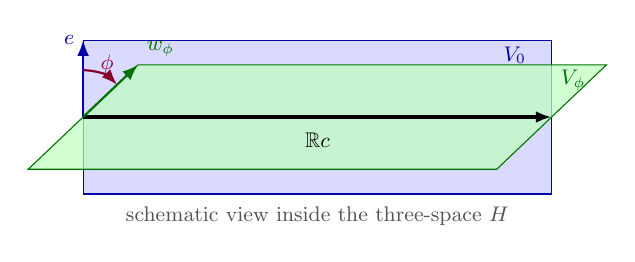
\begin{tikzpicture}[scale=0.85,transform shape,font=\small]
  \coordinate (O) at (0,0);
  \coordinate (C) at (7.0,0);
  \coordinate (E) at (0,1.15);
  \coordinate (W) at (0.82,0.78);

  \fill[blue!20,opacity=0.72]
    ($(O)-(E)$)--($(C)-(E)$)--($(C)+(E)$)--($(O)+(E)$)--cycle;
  \draw[blue!65!black]
    ($(O)-(E)$)--($(C)-(E)$)--($(C)+(E)$)--($(O)+(E)$)--cycle;
  \fill[green!25!white,opacity=0.72]
    ($(O)-(W)$)--($(C)-(W)$)--($(C)+(W)$)--($(O)+(W)$)--cycle;
  \draw[green!45!black]
    ($(O)-(W)$)--($(C)-(W)$)--($(C)+(W)$)--($(O)+(W)$)--cycle;

  \draw[-{Latex[length=2mm]},black,very thick] (O)--(C)
    node[midway,below=3pt] {$\mathbb Rc$};
  \draw[-{Latex[length=2mm]},blue!65!black,thick] (O)--(E)
    node[left] {$e$};
  \draw[-{Latex[length=2mm]},green!45!black,thick] (O)--(W)
    node[above right] {$w_\phi$};
  \draw[-{Latex[length=2mm]},purple!70!black,thick]
    (0,0.70) arc[start angle=90,end angle=43.55,radius=0.70];
  \node[purple!70!black] at (0.36,0.79) {$\phi$};
  \node[blue!65!black] at (6.45,0.92) {$V_0$};
  \node[green!45!black] at (7.32,0.55) {$V_\phi$};
  \node[gray!65!black] at (3.5,-1.48)
    {schematic view inside the three-space $H$};
\end{tikzpicture}
\caption{Twist freedom in the valid $5+2+5$ construction.  The planes
$V_0,V_\phi\subset H$ share $\mathbb Rc$; twisting the rotation plane changes
optional cross-distances while preserving every required unit edge.}
\label{fig:twist-family}
\end{figure}

To certify noncongruence without retaining any labels, use the symmetric
distance invariant
\[
 I(P)=\sum_{\{x,y\}\subset P}\lVert x-y\rVert^6.
\]
In the standard centered coordinates
$q_i=(e_i-\frac15\mathbf1)/\sqrt2$ in the sum-zero hyperplane of
$\mathbb R^5$, with the Gram--Schmidt convention just described, exact
calculation gives
\[
 I(P_0)=\frac{4544767}{24000},
 \qquad
 I(P_{\pi/6})=\frac{4907693}{25920}.
\]
The invariant values differ, so $P_0$ and $P_{\pi/6}$ are noncongruent.
Moreover, \eqref{eq:varying-cross-distance} ranges over an interval, whereas
a fixed unlabelled twelve-point set has only $\binom{12}{2}=66$ pair
distances.  Thus the family contains continuously many congruence classes.

\end{document}
